%%%%%%%%%%%%%%%%%%%%%%%%%%%%%%%%%%%%%%%%%%%%%%%%%%%%%%%%%%%%%%%%%%%%%%%%%%%%%%%%%%%%%%%%%%%%%%%%%%%%%%
%
%   Filename    : chapter_5.tex 
%
%   Description : This file will contain your Results and Analysis.
%                 
%%%%%%%%%%%%%%%%%%%%%%%%%%%%%%%%%%%%%%%%%%%%%%%%%%%%%%%%%%%%%%%%%%%%%%%%%%%%%%%%%%%%%%%%%%%%%%%%%%%%%%

\Section{Results and Analysis}
\label{sec:resultsandanalysis}

This chapter discusses the overall quality of the extracted relations. It also describes the results and the methodology in evaluating them.

\subsection{Methodology}
\label{sec:methodology}

This section details the strategies employed in evaluating the quality and completeness of the extracted relations.

\subsubsection{Quantitative Evaluation}

In order to evaluate the accuracy of the relations extracted, a gold standard was created. The gold standard consists of 3 stories selected from the \textit{MODIFIED} corpora. Each were manually tagged with the appropriate relations. The rules in tagging the relations for the gold standard was independent from the rules followed in this research. For example, the gold standard has tagged relations that span more than 2 sentences. This was not the same for the automatically extracted relations. Lastly, only unique relations are tagged.

After completing the gold standard, the unique automatically extracted relations from the same stories were used for comparison. The extractions' precision, recall and F-measure were computed to come up with the accuracy.

\subsubsection*{Selected Stories}

Each story used in developing the gold standard was selected for different reasons. Shown below are the titles of the stories and a brief description.

\begin{enumerate}
\item \textbf{Everybody Cries} - This was from the \textit{Little Life Lessons} story group. It has 86 lines with a mix of simple and complex sentences. It's target audience are 4-7 year old children. It was selected for its length and complexity. Aside from this, it was determined almost all target relation types, except for \textit{MadeOf}, can be tagged in the story. 
\item \textbf{Start School} - This was from the \textit{Topsy Tim} story group. It has 39 lines with a mix of simple and complex sentences. It's target audience are 4-7 year old children. It was selected for its complexity and target age group. 
\item \textbf{Hopsalot's Garden} - This was from the \textit{Jumpstart} story group. It has 22 lines of mostly simple sentences. It's target audience are 8-10 year old children. It was selected for its simplicity and target age group. 
\end{enumerate}

\subsubsection*{Metrics}

In determining the accuracy and completeness of extractions, 3 metrics were used. These are precision, recall and F-measure. Precision shows the probability that an extracted relation is a true positive and expected to be extracted from the stories. 

\[Precision = \frac{extracted relations \cap expected relations}{extracted relations}\]

Recall shows the probability that an expected extraction from the gold standard is actually extracted from the stories. It will show how complete the automatic extractions are.

\[Recall = \frac{extracted relations \cap expected relations}{expected relations}\]

F-measure is the weighted average of precision and recall. In this evaluation, the balanced F-measure is computed. The best value is 1 and the worst is 0. This will determine the test's accuracy.

\[F = 2 \cdot \frac{precision \cdot recall}{precision + recall}\]

The final values were rounded off to 2 decimal places.

\subsubsection{Story Evaluation}

In order to validate the quality of the extracted relations, they were used to generate stories in Picture Books. First, Picture Books was examined to determine which themes can be used. Then, the target relations extracted from the \textit{RAW} and \textit{MODIFIED} corpora were evaluated to see whether any of them can be easily inserted into the existing Picture Books ontology. Additional relations were manually added by the researcher for the target relations which did not have valid extractions from either corpora. Then, the Picture Books databases were manually updated with a select number of valid extractions, as well as the additional ones. 

\subsubsection*{Examining the Picture Books Themes}
\label{sec:examinethemes}

Aside from checking the valid extractions that can be used for testing, the themes of Picture Books were also examined. There are two motivations for this. First, the researcher would like to determine which among the themes can be used for testing. And secondly, he would like to map which target relation types can be tested for each theme selected.

After carefully tracing the ontology accesses and searches within the 15 different themes, five (5) were identified. Table \ref{tab:mapthemerel} shows the themes selected for testing with the mapped target relation types.

\begin{table}[H]   %t means place on top, replace with b if you want to place at the bottom
\centering
\caption{Mapping of Picture Books Themes with Target Relation Types} \vspace{0.25em}
\begin{tabular}{|p{5cm}|p{5cm}|} \hline
\textbf{Theme ID and Lesson} & \textbf{Mapped Target Relation Types} \\ \hline
THME0001: Take Bath			& usedFor \\ \hline
THME0003: Be Careful		& isA, capableOf, effectOf, propertyOf \\ \hline
THME0012: Be Honest			& isA, capableOf, effectOf, propertyOf \\ \hline
THME0005: Be Neat			& eventForGoalEvent \\ \hline
THME0015: Be Brave			& effectOfIsState \\ \hline
\end{tabular}
\label{tab:mapthemerel}
\end{table}  

After examination, only 7 target relation types were possible to be tested using the existing Picture Books themes.

\subsubsection*{Grouping Target Relation Types}
\label{sec:grouprel}

Since only 7 target relation types can be tested by branching the existing ontology accesses and searches in the existing themes (See Section \ref{sec:examinethemes}), another group was created. This includes the 9 remaining target relation types which were not present in any of Picture Books' existing themes. A summary of the grouping is shown in Table \ref{tab:relgroups}.

\begin{table}[H]   %t means place on top, replace with b if you want to place at the bottom
\centering
\caption{Target Relation Type Groups} \vspace{0.25em}
\begin{tabular}{|p{5cm}|p{5cm}|} \hline
\textbf{Group A: Used in existing themes} & \textbf{Group B: Not used in existing themes} \\ \hline
isA, capableOf, propertyOf, effectOf, effectOfIsState, usedFor, eventForGoalEvent	& locationOf, partOf, madeOf, eventForGoalState, oftenNear, happens, hasRole, roleResponsibleFor, owns \\ \hline
\end{tabular}
\label{tab:relgroups}
\end{table}

\emph{Group A Relations}

For this group, 9 new lexicon entries and 12 new concepts were added into the database. The discrepancy was due to the words already existing in the lexicon but not as concepts to be used for ontology searches. Then, forty-one (41) new ontology entries were added to branch from existing ontology searches. Shown in Figure \ref{fig:altpath} is a sample alternative path created for this study. This is for author goal AUTH0026 of theme THME0003 (Be Careful).

\begin{figure}[h]                %-- use [t] to place figure at top, [b] to place at the bottom
   \centering                    %-- use this to center the figure
   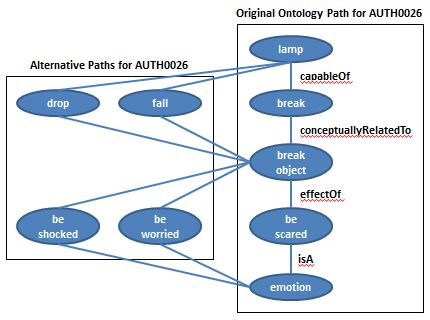
\includegraphics{altpath.jpg}      %-- include image file named as "sinag1.eps" 
   \caption{Alternative Path for AUTH0026}
    \label{fig:altpath}
\end{figure}

From the figure, there were 4 new concepts added and 8 new relations (2 \textit{IsA}, 2 \textit{ConceptuallyRelatedTo}, 2 \textit{EffectOf} and 2  \textit{CapableOf}). Though the relation \textit{ConceptuallyRelatedTo} is not really a target relation for this study, such entries were still created to maintain the path going to the last node (\textit{emotion}). 

However, as an exceptional case in this group of relations, the \textit{EffectOfIsState} relation was configured differently. Aside from the additional lexicon entries, concepts and ontology entries, 2 new author goals and 2 new story plot trackers were created. The new story plot trackers were then added as alternative Solutions to the theme THME0015 (Be Brave). This is all due to the difference in accessing the \textit{EffectOfIsState} in the author goal AUTH0056. Figure \ref{fig:altpatheffectofisstate} shows how the relation was accessed in the path. Instead of accessing the relation in the middle of the path, it was done at the end which was explicitly indicated in the definition of the author goal AUTH0056. This means there is no way to randomly select a new concept. 

\begin{figure}[h]                %-- use [t] to place figure at top, [b] to place at the bottom
   \centering                    %-- use this to center the figure
   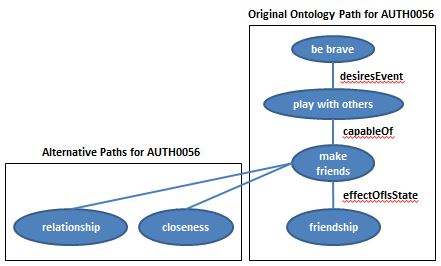
\includegraphics{altpatheffectofisstate.jpg}      %-- include image file named as "sinag1.eps" 
   \caption{Alternative Path for AUTH0056}
    \label{fig:altpatheffectofisstate}
\end{figure}

Appendix E shows all the additional entries in the Picture Books lexicon and ontology.

\emph{Group B Relations}

Because Group B relations did not exist in the current version of Picture Books' ontology, author goals were created to show the relations in the generated stories. 16 new lexicon entries and 20 new concepts were added into the database. Then, 27 new ontology entries were added. Finally, 9 new author goals were created and inserted as additional author goals of story plot tracker SPAT0004. 

For this group of relations, the theme THME0001 (Take Bath) was used. Each relation type had 2 representative sentences created and were included in the final story generated. None of the concepts and sentences were made coherent to the rest of the story. Appendix E shows all the additional entries in the Picture Books lexicon and ontology.

\subsubsection*{Selected Relations}
\label{sec:selectedrelations}

Out of all the extracted relations from the \textit{RAW} and \textit{MODIFIED} corpora, only 6 relations were used and all of them are \textit{PartOf} relations. The rest of the relations used for testing were manually created. 

Group A needed extracted relations that are related to the themes selected as they are embedded in the ontology searches and accesses. But none of the extracted relations that fall under this group were coherent to any of the themes. \textit{EffectOfIsState} was also not extracted. Thus, it was decided to just create new relations that would be coherent to the rest of the stories. 

Group B, on the other hand, did not require the extracted relation to be coherent to the theme \textit{Take Bath} because that was not the intention. But because \textit{MadeOf} and \textit{OftenNear} were not extracted at all and \textit{EventForGoalState}, \textit{Happens}, \textit{HasRole}, \textit{Owns} and \textit{RoleResponsibleFor} did not have valid extractions, manual entries were also created.

\subsection{Extraction Analysis}
\label{sec:extractionanalysis}

\subsubsection{Accuracy and Completeness}

\begin{table}[H]   %t means place on top, replace with b if you want to place at the bottom
\centering
\caption{Gold Standard Evaluation Results} \vspace{0.25em}
\begin{tabular}{|p{3cm}|p{2cm}|p{2cm}|p{1cm}|p{1.5cm}|p{1cm}|p{1cm}|p{1cm}|} \hline
\textbf{Stories} & \textbf{Gold Standard} & \textbf{Extraction} & \textbf{Delta} & \textbf{Correct} & \textbf{P} & \textbf{R} & \textbf{F} \\ \hline
Overall (RAW) & 663 & 615 & -48 & 212 & 0.34 & 0.32 & 0.33 \\ \hline
Overall (MODIFIED) & 663 & 662 & -1 & 241 & 0.36 & 0.36 & 0.36 \\ \hline
Everybody Cries (RAW) & 456 & 392 & -64 & 137 & 0.35 & 0.30 & 0.32 \\ \hline
Everybody Cries (MODIFIED) & 456 & 410 & -46 & 156 & 0.38 & 0.34 & 0.36 \\ \hline
Start School (RAW) & 139 & 150 & 11 & 47 & 0.31 & 0.34 & 0.33 \\ \hline
Start School (MODIFIED) & 139 & 173 & 34 & 54 & 0.31 & 0.39 & 0.35 \\ \hline
Hopsalot's Garden (RAW) & 68 & 73 & 5 & 28 & 0.38 & 0.41 & 0.40 \\ \hline
Hopsalot's Garden (MODIFIED) & 68 & 79 & 11 & 31 & 0.39 & 0.46 & 0.42 \\ \hline
\end{tabular}
\label{tab:goldsum}
\end{table}

In this evaluation, the precision, recall and F-measure values were analyzed to determine whether the approach used in automatically extracting the  relations yielded accurate and complete extractions.

Shown in Table \ref{tab:goldsum} are the results after comparing the automatically extracted relations from both the raw and modified versions of the stories to the gold standard. The \textit{Gold Standard} column shows the number of tagged relations in the gold standard for a specific story. The value is the same for the \textit{RAW} and \textit{MODIFIED} rows of the same story. The \textit{Extraction} column shows the number of automatically extracted relations using this research's approach. It is followed by the \textit{delta} which show whether there was over-extraction or under-extraction. The \textit{Correct} column shows the number of correct automatically extracted relations after comparing with the gold standard. Columns \textit{P}, \textit{R} and \textit{F} show the precision, recall and F-measure values, respectively.

Overall, the \textit{RAW} and \textit{MODIFIED} stories garnered 0.33 and 0.36, respectively, for their accuracy. The increase for the \textit{MODIFIED} stories give a positive indication that the modifications done on the corpus has helped in improving the accuracy of the extractor. However, these values are still low and does not even pass the half way point. Despite cleaning the data and making sure that proper information and relations are extracted, the templates are still lacking. Appendix G shows the detailed results per relation per story.

\subsubsection*{Excess and Deficient Extractions}

Focusing on the \textit{delta} values alone, it is noticeable that there is no overall trend in the number of automatic extractions done. Only the \textit{Everybody Cries} story had less extractions while the rest of the stories had increases.  

Going into specific relation types, there are three consistent ones. \textit{CapableOf} and \textit{EffectOfIsState} show consistent decreases while \textit{PropertyOf} shows consistent increases. In the case of \textit{CapableOf}, one main reason is that the action done is not always detected. Its extraction template immediately looks for an adjacent verb as its capable action. If there are modal or other words between the doer and the action in a sentence, no relation will be extracted. Such is also the case for sentences that have complex verb phrase structures. Here is a sample sentence from \textit{Everybody Cries}:

\begin{verse}
\itshape
While he pretends to catch, throw, and bat, Bear bumps into Pig's swing.
\end{verse}

In the gold standard, there were 4 \textit{CapableOf} relations extracted from that sentence:

\begin{verse}
\itshape
CapableOf(Bear,pretend to catch) \\ 
CapableOf(Bear,pretend to throw)\\
CapableOf(Bear,pretend to bat)\\
CapableOf(Bear,bump)\\
\end{verse}

The \textit{pretends to catch, throw, and bat} were divided into 3 separate relations. But in the current templates, this is not handled.

For \textit{EffectOfIsState}, there is a consistent 100\% decrease in the number of extractions as compared to the gold standard. This was due to the fact that the template requires an adjective as an effect state but the ANNIE part-of-speech tagger is not able to tag them accurately.

Lastly, \textit{PropertyOf} relations showed the greatest increase among the relation types. But in this case, the fault lies on the way the transducer was designed to extract this kind of relation. In its template, the transducer is supposed to relate an adjective to an adjacent noun. But unlike the rest of the relations, the transducer does not stop until all possible nouns are related to it.

\subsubsection*{Complex and Long Stories}

In Table \ref{tab:goldsum}, the stories are ordered based on the length and complexity of its sentences. \textit{Everybody Cries} has the most number of lines and the most complex sentences. \textit{Hopsalot's Garden} has the least number of lines and the simplest sentences. If this is observed alongside their \textit{precision}, \textit{recall} and \textit{F-measure} values, there is a seemingly upward trend. The length of the story and complexity of the sentences are indirectly proportional to the accuracy of extraction. As the complexity of the sentences (with the introduction of more clauses) and the number of lines increases (longer stories), the extractor suffers from lower accuracy.

\subsubsection*{Correct and Complete Extractions}

Overall, the extractor yielded fairly low \textit{precision}, \textit{recall} and \textit{F-measure} values. This shows that the templates used, despite their generalized nature to accommodate a number of patterns, were not able to extract an acceptable number of valid relations. And because of this, the templates were not successful in extracting all the expected valid relations from the stories. 

For those relation types which were able to extract more than the expected, the way the transducer was designed to extract them did not help in improving the quality of relations. It introduced more nuisance relations than expected. Another contributing factor would be their loose and highly generalized templates. As for those that had lower extractions than the gold standard, their templates may have been a bit stricter but it also caused the extractor to miss a lot of valid extractions. 

And for most relation types, another reason would be their limitation to be extracted from a single sentence only. The gold standard had a lot of inferred and implied tagged relations that span even more than 2 sentences. These would be impossible to extract using the current approach. Also, almost all gold standard relations were tagged not using much of the defined indicators in this study.

However, there was a bright spot amongst the relation types. The \textit{Owns} relation type was consistent in getting \textit{precision} and \textit{recall} values ranging from 0.48 to even 0.77. It only got a \textit{precision} of 0.48 in \textit{Everybody Cries} while in the other 2 stories, values were always above 0.62. Though in a broader sense, the scores are still low and not acceptable, it is worth noting how this relation type consistently bested the other relations in terms of extractions. 

First, \textit{Owns} relations are easy to distinguish in a sentence. When a possessive noun or pronoun is present, it is highly likely that the noun adjacent to it would constitute your second concept. Also, this relation type, unlike most, is almost always found within a sentence. And if it is within a span of text, there are only a few indicators possible and the ways it can be expressed are limited. Lastly, its templates are simpler and straightforward. There was not a lot of generalization done because there are not a lot of ways that an \textit{Owns} relation is manifested in a sentence. However, it cannot handle possessions (second concept) that have more than 1 word specially when adjectives are used. For example, the relation \textit{Owns(Bear,first game)} was not extracted because the template was immediately looking for a noun. The presence of the adjective \textit{first} hindered this extraction.  

\subsubsection*{Low Correct Extractions}

In this section, only the \textit{Everybody Cries} story is considered since it was the only story that have almost all relation types tagged in the gold standard. 

Though the extractor was able to identify relations for almost all types except for \textit{MadeOf}, \textit{EffectOfIsState} and \textit{OftenNear}, there were some relation types that have very low correct extraction while some did not have any correct extractions at all. First in the list would be the \textit{IsA} relation. In the gold standard, all relations of this type were implied and spans across sentences. The use of indicators were also not apparent. Here is an example:

\begin{verse}
\itshape
Puppy likes to have a good breakfast before school. \\
This morning he has no time for cereal, toast, or juice.\\
\end{verse}

In the gold standard, it was able to identify the following \textit{IsA} relations:

\begin{verse}
\itshape
IsA(cereal,breakfast)\\
IsA(juice,breakfast)\\
IsA(toast,breakfast)\\
\end{verse}

The current \textit{IsA} templates cannot handle this since it is limited to a sentence and it highly relies on indicators.

Next, \textit{PartOf} relations had a very low turnout of correct relations because of its similarity to \textit{Owns}. One of its template uses possessive nouns or pronouns to signal its presence. However, the extractor is only able to differentiate it from an \textit{Owns} extraction when the second concept or the possession is a body part. In cases like \textit{car's wheel} and \textit{building's glass windows}, it wasn't able to identify the \textit{PartOf} relation. Instead, these are incorrectly tagged as \textit{Owns}.

\textit{EventForGoalEvent} is another case of confusion. In most cases, these types of relations are identified by the extractor as \textit{EffectOf} because of the similarity in structure when apparent in a text. Because desires are not always explicitly shown, the extractor had a difficult time differentiating this relation from \textit{EffectOf} which can accept just events as cause and effect if there are no indicators used. Another reason why this relation had a low turnout was that despite being able to extract from 2 sentences, most of the gold standard relations were extracted beyond 2 sentences. Here is an excerpt from the story:

\begin{verse}
\itshape
They will all share their lunches with Puppy.\\
Puppy's friends pass him bits from their lunches. \\
Hippo shares his sandwich with Puppy. \\
Bear gives him some crackers. \\
Mouse shares her pudding. \\
Cat gives him part of her apple.\\
\end{verse}

The gold standard was able to identify the following relations:

\begin{verse}
\itshape
EventForGoalEvent(give cracker,share lunch)\\
EventForGoalEvent(give part of apple,share lunch)\\
EventForGoalEvent(pass bits,share lunch)\\
EventForGoalEvent(share pudding,share lunch)\\
EventForGoalEvent(share sandwich,share lunch)\\
\end{verse}

In this specific example, the relations were present even if they were 4 sentences apart. Clearly, the extractor was not able to handle that. Aside from that, there was no clear indication in the first sentence that \textit{share lunch} was the desire of Puppy's friends. 

The \textit{UsedFor}, \textit{Happens} and \textit{HasRole} relations also had zero correct extractions. \textit{UsedFor} was not able to correctly extract the expected relations because its templates were always expecting an indicator. But in the story, all \textit{UsedFor} instances did not use indicators. Here is an example:

\begin{verse}
\itshape
She is writing on the blackboard and does not turn around to look at Puppy.
\end{verse}

The gold standard was able to identify the relation \textit{UsedFor(blackboard,write)} but this was not present in the actual extractions. The existing  templates should have been able to identify this if no indicators were expected.

As for the \textit{Happens} relation, the extractor always extracted a relation when the \textit{today} time indicator was used in a sentence. But in the gold standard, \textit{today} was not considered a valid time indicator as it is vague and does not really give a valid time within a day.

\textit{HasRole} is one of those relations that is quite rare and hard to find in a story. In the gold standard, there was only 1 \textit{HasRole} found and it is \textit{HasRole(Miss Hen,teacher)}. This was not extracted using the extractor. First, the templates are looking for indicators and certain structures for it to identify the relation. But in this case, the correct relation was identified by inferring from the actions done by \textit{Miss Hen} in the story. The role was also not mentioned in the story. The gold standard used the following actions in determining the \textit{teacher} role for \textit{Miss Hen}: \textit{ask the class}, \textit{collect assignment}, \textit{start class} and \textit{write on the blackboard}. These are specific actions that are done by a teacher which is why the said role was related to the character.

Lastly, the \textit{OftenNear} relation did not have any correct extractions because of insufficient indicators. The only \textit{OftenNear} relation identified in the gold standard was \textit{OftenNear(house,sidewalk)}. This was identified using the word \textit{along} which was not included as one of the \textit{OftenNear} indicators. Had it been added in the first place, the said relation would have existed as part of the extractions.  

\subsubsection{Uniqueness and Redundancies}

In this evaluation, the number of unique extractions were analyzed to determine whether the modifications created more relations valid for extraction. Also, duplicate or redundant extractions are also analyzed to see whether they were reduced after modification.

There was a total of 13,871 unique relations extracted from the \textit{RAW} and \textit{MODIFIED} corpora. Tables \ref{tab:modifiedtotal} and \ref{tab:rawtotal} show the breakdown of numbers for each group of stories in each corpora.

\begin{table}[H]   %t means place on top, replace with b if you want to place at the bottom
\centering
\caption{Raw Corpus: Number of Unique and Redundant Relations Extracted} \vspace{0.25em}
\begin{tabular}{|p{4cm}|p{3cm}|p{3cm}|} \hline
\textbf{Story Group} & \textbf{Unique} & \textbf{Redundant} \\ \hline
Jumpstart & 644 & 194 \\ \hline
Winnie the Pooh & 394 & 94 \\ \hline
Topsy Tim & 684 & 215 \\ \hline
Little Life Lessons & 4977 & 2017 \\ \hline
\textbf{TOTAL} & \textbf{6699} & \textbf{2520} \\ \hline
\end{tabular}
\label{tab:rawtotal}
\end{table}

\begin{table}[H]   %t means place on top, replace with b if you want to place at the bottom
\centering
\caption{Modified Corpus: Number of Unique and Redundant Relations Extracted} \vspace{0.25em}
\begin{tabular}{|p{4cm}|p{3cm}|p{3cm}|} \hline
\textbf{Story Group} & \textbf{Unique} & \textbf{Redundant} \\ \hline
Jumpstar
t & 729 & 206 \\ \hline
Winnie the Pooh & 436 & 137 \\ \hline
Topsy Tim & 747 & 341 \\ \hline
Little Life Lessons & 5260 & 2621 \\ \hline
\textbf{TOTAL} & \textbf{7172} & \textbf{3305} \\ \hline
\end{tabular}
\label{tab:modifiedtotal}
\end{table}

From these numbers, it is evident that the \textit{Modified} corpus had 473 more relations extracted than the \textit{Raw} corpus. This suggests that the modifications done introduced new concepts, thus allowing the application to extract more unique relations. These modifications may have also introduced more redundant relations as the number increased by 785. This was even more than the increase in unique relations. Here are sample passages from \textit{CJ and the Mysterious Map}:

\begin{verse}
\itshape
``And how do you suggest we get up there?" asked Edison.\\
``What are you doing?" asked Edison.\\
\end{verse}

These are non-adjacent sentences from the story. After running this in the extraction tool, they yielded zero extractions. Then they were modified to this:

\begin{verse}
\itshape
Edison asked CJ some suggestions.\\
Edison asked what CJ is doing.\\
\end{verse}

Now, each sentence was able to produce 2 new \textit{CapableOf} extractions. However, both of them are \textit{CapableOf(Edison,ask)}. And after examining the modified story, there were more sentences of this structure that yielded the same relation. 

In terms of relations, Table \ref{tab:reltotal} shows the breakdown of extracted relations per corpora. The delta after modification is also shown. 

\begin{table}[H]   %t means place on top, replace with b if you want to place at the bottom
\centering
\caption{Number of Relations Extracted per Corpus} \vspace{0.25em}
\begin{tabular}{|p{4.5cm}|p{2cm}|p{2cm}|p{2cm}|} \hline
\textbf{Relations} & \textbf{Raw} & \textbf{Modified} & \textbf{Delta} \\ \hline
IsA & 191 & 228 & 37 \\ \hline
PropertyOf & 2700 & 2857 & 157 \\ \hline
PartOf  & 71 & 84 & 13 \\ \hline
MadeOf & 0 & 0 & 0 \\ \hline
EventForGoalEvent & 481 & 580 & 99 \\ \hline
EventForGoalState & 31 & 37 & 6 \\ \hline
EffectOf & 1258 & 1196 & -62 \\ \hline
EffectOfIsState & 0 & 0 & 0 \\ \hline
CapableOf & 980 & 1193 & 213 \\ \hline
OftenNear & 0 & 0 & 0 \\ \hline
LocationOf & 136 & 137 & 1 \\ \hline
UsedFor & 228 & 232 & 4 \\ \hline
Happens & 38 & 34 & -4 \\ \hline
HasRole & 11 & 14 & 3 \\ \hline
RoleResponsibleFor & 11 & 13 & 2 \\ \hline
Owns & 562 & 565 & 3 \\ \hline
\end{tabular}
\label{tab:reltotal}
\end{table}

In a relational level, almost all relations experienced an increase in the number of extractions except for \textit{EffectOf} and \textit{Happens}. Again, although the delta is not significant in number, it suggests that the modifications avoided the extraction of possible relations. Here is an  extracted relation from the \textit{Raw} corpus that is not included as an extracted relation in the \textit{Modified} corpus:

\begin{verse}
\itshape
EffectOf(said,not forgive and forget)
\end{verse}

It was extracted from this passage from \textit{Forgive and Forget} of the \textit{Winnie the Pooh} story group:

\begin{verse}
\itshape
``Rabbit, I think Tigger is very sorry," Pooh said. ``Will you not forgive and forget?"
\end{verse}

This specific sentence was modified to this:

\begin{verse}
\itshape
Pooh thinks Tigger is very sorry. Pooh asks Rabbit if he can forgive and forget.
\end{verse}

In this example, the verb \textit{said} was removed after modification, thus avoiding the possibility of another relation being extracted. It seems that modifications, such as this, improved the result for the \textit{Modified} corpus because the relation is not really a valid and logical extraction. However, the possibility that valid extractions may also be omitted in the process cannot be discounted.

\subsubsection{Zero Extraction}

From the same table, it is important to note that the \textit{EffectOfIsState}, \textit{MadeOf} and \textit{OftenNear} relations had 0 extractions from either corpora. This was caused by their high dependence on indicators, incorrect part-of-speech tags and limitation on the number of sentences it can extract from. 

\subsubsection{Quality}

In terms of extraction quality, there are some relations which may have been incorrectly extracted or which may not be extracted at all because of incorrect tags. For instance, this relation was extracted from the \textit{Jumpstart} story group:

\begin{verse}
\itshape
EffectOf(went on full speed,shocked)
\end{verse}

The extraction seems valid from first glance, but looking at its original passage may suggest otherwise. Shown below is the modified passage from \textit{Just in time}. Instead of \textit{EffectOf}, a better extraction could have been \textit{EffectOfIsState} since \textit{being shocked} is an implied state. 

\begin{verse}
\itshape
Frankie went on full speed.\\
Hopsalot was shocked.
\end{verse}

Other incorrect extractions were due to a different part-of-speech information tagged to the concept and the lack of additional semantic information.

Lastly, it is important to note that for event relations like \textit{EffectOf} and \textit{EventForGoalEvent}, the extracted relations seem to be longer and more specific because the extractor uses whole phrases as concepts. This may be different from the concepts of Picture Books that are more generalized. Here are some example extractions:

\begin{verse}
\itshape
EffectOf(looked at the map,checked the wind)\\
EffectOf(pours something into the volcano,stopped him)\\
EventForGoalEvent(called everyone,go to the ship)
\end{verse}

For a more detailed look in the extraction results, kindly refer to Appendix D.

\subsection{Story Analysis}
\label{sec:storyanalysis}

Overall, the new relations were used accordingly. They were randomly selected and used interchangeably with the original relations. But the sentences generated were fairly acceptable. There are cases wherein the sentence is grammatically incorrect. For example, here is an original story generated for the \textit{Be Careful} theme:

\begin{alltt}
\textbf{Edward the elephant learns to be careful.}

[1]  The morning was sunny.
[2]  Edward the elephant was in the dining room.
[3]  He played near breakable glass of water.
[4]  Daddy Sam told Edward to be careful.
[5]  Edward continued to play glass of water near.
\underline{\emph{\textbf{[6]  He broke it.}}}
\underline{\emph{\textbf{[7]  Edward was scared.}}}
[8]  He hid away from Daddy Sam.
\underline{\emph{\textbf{[9]  Daddy Sam saw that glass of water was broken.}}}
[10] Daddy Sam called Edward.
[11] Daddy Sam told Edward that he should have obeyed.
[12] He felt sorry.
[13] Daddy Sam cleaned up glass of water.
[14] Edward helped Daddy Sam to clean up.
[15] Daddy Sam reminded Edward to be careful.
[16] Being careful is important.
[17] From that day onwards, Edward always was careful.
\end{alltt}

This used the original relations of Picture Books. The highlighted lines show the sentences where the changes should happen. Shown below is another story using the same characters and objects as the story above. This time, the highlighted sentences are using different concepts based on the new additions to the lexicon and ontology.

\begin{alltt}
\textbf{Edward the elephant learns to be careful.}

[1]  The afternoon was sunny.
[2]  Edward the elephant was in the dining room.
[3]  He played near breakable glass of water.
[4]  Mommy Edna told Edward to be careful.
[5]  Edward continued to play glass of water near.
\underline{\emph{\textbf{[6]  Edward fell it.}}}
\underline{\emph{\textbf{[7]  Edward was worried.}}}
[8]  He hid away from Mommy Edna.
\underline{\emph{\textbf{[9]  Mommy Edna saw that glass of water was cracked.}}}
[10] Mommy Edna called Edward.
[11] Mommy Edna told Edward that he should have obeyed.
[12] Edward felt sorry.
[13] Mommy Edna cleaned up glass of water.
[14] Edward helped Mommy Edna to clean up.
[15] She reminded Edward to be careful.
[16] Being careful is important.
[17] From that day onwards, Edward always was careful.
\end{alltt}

In line 6, instead of the usual action \textit{broke}, the story now uses \textit{fell}. However, the new sentence should have been ``It fell" or ``The glass of water fell." Since the relation used here is \textit{CapableOf(lamp,fall)}, it also logical to note that the \textit{lamp} can be the agent of the action instead of always being the character. 

Another new story worth pointing out is this:

\begin{alltt}
\textbf{Edward the elephant learns to be honest.}

[1]  The morning was warm.
[2]  Edward the elephant was in the dining room.
[3]  He played near breakable glass of water.
\underline{\emph{\textbf{[4]  Edward fell glass of water.}}}
[5]  He was worried.
[6]  Mommy Edna saw that glass of water was smashed.
[7]  Edward told Mommy Edna that Porky the pig broke glass of water.
[8]  He was sad.
[9]  Porky cried.
[10] Edward felt guilty.
\underline{\emph{\textbf{[11] Edward told Mommy Edna that he dropped glass of water.}}}
[12] Mommy Edna told Edward that he should have been honest.
[13] He apologized to Mommy Edna.
[14] Edward apologized to Porky.
[15] Mommy Edna told Edward to be honest.
[16] Mommy Edna told Edward that being honest is good.
[17] From that day onwards, Edward always was honest.
\end{alltt}

In this story, highlighted are the sentences using the \textit{CapableOf} relations with \textit{lamp} as the parent concept, \textit{CapableOf(lamp,fall)} and \textit{CapableOf(lamp,drop)}. Though it is valid to use both, having them in just one story creates inconsistencies. In line 4, it was already mentioned that the glass of water fell. And since the word \textit{fell} was used, there is an implication of an accident which creates a different dimension to the story. Now in line 11, though Edward is already admitting his fault, he suddenly said \textit{dropped} instead of the initial \textit{fell}. This might create confusion as dropping something makes the act intentional whereas when it fell, Edward may or may not have caused the action. When the act \textit{fell} was used in line 4, it expected that the same act is confessed in line 11.

Lastly, there are a number of instances where incorrect relations are picked up by Picture Books in doing ontology accesses and searches. As a result, incorrect sentences are generated. For example, in the story \textit{Roy the chicken learns to take bath.} shown below, lines 9 and 10 are produced using the same relation, \textit{OftenNear}. They also have the same parent concept which is \textit{school}. Line 9 has a correct child concept but Line 10 does not. Instead of either \textit{clinic}, \textit{mall} or \textit{market}, it used \textit{generic}. After examining the ontology, \textit{generic} is the child concept when the relation is \textit{PropertyOf}. This shouldn't be the case. 

The reason why this happens is because Picture Books searches its ontology not by the name of the relation but by its category. In the ontology, both \textit{OftenNear} and \textit{PropertyOf} are under the category \textit{spatial}. This causes Picture Books to not only randomize among \textit{OftenNear} relations but also including the \textit{PropertyOf} relation.

\begin{alltt}
[1]  Toys were the bedroom.
[2]  Playing is the playground.
[3]  An oak had trunk.
[4]  A person had a toe.
[5]  A book had paper.
[6]  It had ink.
[7]  Playing is dirty.
[8]  It was healthy.
\underline{\emph{\textbf{[9]  The school was the market.}}}
\underline{\emph{\textbf{[10] It was generic.}}}
[11] Eating dinner is the evening.
[12] Going to the school is the morning.
[13] A fireman was rescuing.
[14] A librarian was organizing.
[15] Daddy Sam had a ball.
[16] He had the tricycle.
[17] From then on, Roy always took the bath.
\end{alltt}

Another example is with the same story but lines 11 and 12 are changed to the following:

\begin{alltt}
[11] Eating dinner is the evening.
\underline{[12] Going to the school is \emph{\textbf{saying goodbye}}.}
\end{alltt}

These two sentences are using the \textit{Happens} relation. But in line 12, the relation \textit{FirstSubeventOf} was used because they are both \textit{event} relations. This happens for ontology accesses that only have 1 argument.

Kindly refer to Appendix F for all the stories generated in this phase.









